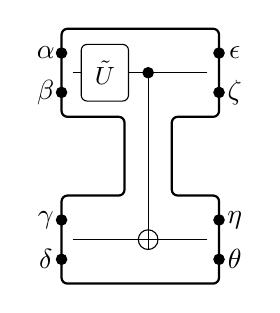
\begin{tikzpicture}[yscale=1]

 \begin{scope}[xscale=-1,xshift=-2cm]   
\draw[rounded corners = .75mm,thick] (0cm, -1.618 cm) -- (2 cm, -1.618 cm) -- (2cm, -.5 cm) -- (1.2cm, -.5 cm) -- (1.2 cm,.5cm) -- (2cm, .5cm) -- (2cm, 1.618cm) -- (0cm, 1.618cm) -- (0cm, .5cm) -- (.6cm, .5cm) -- (.6cm, -.5cm) -- (0cm, -.5cm) -- cycle; 
    \draw (.15cm, 1.06cm) -- (1.85cm, 1.06cm); 
 \draw (.15cm, -1.06cm) -- (1.85cm, -1.06cm);
  \draw (.9cm,1.06cm) -- (.9cm,-1.06cm);   
\draw[fill=black] (.9,1.06cm) circle (.66mm); 
 \draw (.9,-1.06cm) circle (1.25mm); 
 \draw (.9,-1.19cm) -- (.9,-.93cm);   
  \draw[rounded corners=.75mm,fill=white] (1.15cm, .7cm) rectangle (1.75cm, 1.42cm); 
 \node at (1.45cm, 1.06cm) {\small $\tilde U$}; 
 \end{scope}   


\node at ( -0.2,1.31) {$\alpha$};
 \draw[fill=black] (0,1.31) circle (.66mm);   

\node at ( -0.2,0.81) {$\beta$};
 \draw[fill=black] (0,0.81) circle (.66mm);   

\node at ( -0.2,-0.81) {$\gamma$};
 \draw[fill=black] (0,-0.81) circle (.66mm);   

\node at ( -0.2,-1.31) {$\delta$};
 \draw[fill=black] (0,-1.31) circle (.66mm);   

\node at (2.2,1.31) {$\epsilon$};
 \draw[fill=black] (2,1.31) circle (.66mm);   

\node at (2.2,0.81) {$\zeta$};
 \draw[fill=black] (2,0.81) circle (.66mm);   

\node at ( 2.2,-0.81) {$\eta$};
 \draw[fill=black] (2,-0.81) circle (.66mm);   

\node at ( 2.2,-1.31) {$\theta$};
 \draw[fill=black] (2,-1.31) circle (.66mm);   

\end{tikzpicture}
\label{fig:GVucnot}